%%%%%%%%%%%%%%%%%%%%%%%%%%%%%%%%%%%
%This is the LaTeX COMMUNICATION template for RSC journals
%Copyright The Royal Society of Chemistry 2014
%%%%%%%%%%%%%%%%%%%%%%%%%%%%%%%%%%%

\documentclass[twoside,twocolumn,9pt]{article}
\usepackage{extsizes}
\usepackage[super,sort&compress,comma]{natbib} 
\usepackage[version=3]{mhchem}
\usepackage[left=1.5cm, right=1.5cm, top=1.785cm, bottom=2.0cm]{geometry}
\usepackage{balance}
\usepackage{widetext}
\usepackage{times,mathptmx}
\usepackage{sectsty}
\usepackage{graphicx} 
\usepackage{lastpage}
\usepackage[format=plain,justification=raggedright,singlelinecheck=false,font={stretch=1.125,small,sf},labelfont=bf,labelsep=space]{caption}
\usepackage{float}
\usepackage{fancyhdr}
\usepackage{fnpos}
\usepackage[english]{babel}
\usepackage{lipsum}
\usepackage{array}
\usepackage{droidsans}
\usepackage{charter}
\usepackage[T1]{fontenc}
\usepackage[usenames,dvipsnames]{xcolor}
\usepackage{setspace}
\usepackage[compact]{titlesec}
%%%Please don't disable any packages in the preamble, as this may cause the template to display incorrectly.%%%
\usepackage[pdftex,unicode,colorlinks, citecolor=blue,%
filecolor=black, linkcolor=blue, urlcolor=black]{hyperref}
\newcommand{\onlinecite}[1]{\hspace{-1 ex} \nocite{#1}\citenum{#1}} 

%\usepackage{epstopdf}%This line makes .eps figures into .pdf - please comment out if not required.

\definecolor{cream}{RGB}{222,217,201}

\begin{document}

\pagestyle{fancy}
\thispagestyle{plain}
\fancypagestyle{plain}{

%%%HEADER%%%
\fancyhead[C]{\includegraphics[width=18.5cm]{head_foot/header_bar}}
\fancyhead[L]{\hspace{0cm}\vspace{1.5cm}\includegraphics[height=30pt]{head_foot/journal_name}}
\fancyhead[R]{\hspace{0cm}\vspace{1.7cm}\includegraphics[height=55pt]{head_foot/RSC_LOGO_CMYK}}
\renewcommand{\headrulewidth}{0pt}
}
%%%END OF HEADER%%%

%%%PAGE SETUP - Please do not change any commands within this section%%%
\makeFNbottom
\makeatletter
\renewcommand\LARGE{\@setfontsize\LARGE{15pt}{17}}
\renewcommand\Large{\@setfontsize\Large{12pt}{14}}
\renewcommand\large{\@setfontsize\large{10pt}{12}}
\renewcommand\footnotesize{\@setfontsize\footnotesize{7pt}{10}}
\renewcommand\scriptsize{\@setfontsize\scriptsize{7pt}{7}}
\makeatother

\renewcommand{\thefootnote}{\fnsymbol{footnote}}
\renewcommand\footnoterule{\vspace*{1pt}% 
\color{cream}\hrule width 3.5in height 0.4pt \color{black} \vspace*{5pt}} 
\setcounter{secnumdepth}{5}

\makeatletter 
\renewcommand\@biblabel[1]{#1}            
\renewcommand\@makefntext[1]% 
{\noindent\makebox[0pt][r]{\@thefnmark\,}#1}
\makeatother 
\renewcommand{\figurename}{\small{Fig.}~}
\sectionfont{\sffamily\Large}
\subsectionfont{\normalsize}
\subsubsectionfont{\bf}
\setstretch{1.125} %In particular, please do not alter this line.
\setlength{\skip\footins}{0.8cm}
\setlength{\footnotesep}{0.25cm}
\setlength{\jot}{10pt}
\titlespacing*{\section}{0pt}{4pt}{4pt}
\titlespacing*{\subsection}{0pt}{15pt}{1pt}
%%%END OF PAGE SETUP%%%

%%%FOOTER%%%
\fancyfoot{}
\fancyfoot[LO,RE]{\vspace{-7.1pt}\includegraphics[height=9pt]{head_foot/LF}}
\fancyfoot[CO]{\vspace{-7.1pt}\hspace{13.2cm}\includegraphics{head_foot/RF}}
\fancyfoot[CE]{\vspace{-7.2pt}\hspace{-14.2cm}\includegraphics{head_foot/RF}}
\fancyfoot[RO]{\footnotesize{\sffamily{1--\pageref{LastPage} ~\textbar  \hspace{2pt}\thepage}}}
\fancyfoot[LE]{\footnotesize{\sffamily{\thepage~\textbar\hspace{3.45cm} 1--\pageref{LastPage}}}}
\fancyhead{}
\renewcommand{\headrulewidth}{0pt} 
\renewcommand{\footrulewidth}{0pt}
\setlength{\arrayrulewidth}{1pt}
\setlength{\columnsep}{6.5mm}
\setlength\bibsep{1pt}
%%%END OF FOOTER%%%

%%%FIGURE SETUP - please do not change any commands within this section%%%
\makeatletter 
\newlength{\figrulesep} 
\setlength{\figrulesep}{0.5\textfloatsep} 

\newcommand{\topfigrule}{\vspace*{-1pt}% 
\noindent{\color{cream}\rule[-\figrulesep]{\columnwidth}{1.5pt}} }

\newcommand{\botfigrule}{\vspace*{-2pt}% 
\noindent{\color{cream}\rule[\figrulesep]{\columnwidth}{1.5pt}} }

\newcommand{\dblfigrule}{\vspace*{-1pt}% 
\noindent{\color{cream}\rule[-\figrulesep]{\textwidth}{1.5pt}} }

\makeatother
%%%END OF FIGURE SETUP%%%

%%%TITLE AND AUTHORS%%%
\twocolumn[
  \begin{@twocolumnfalse}
\vspace{3cm}
\sffamily
\begin{tabular}{m{4.5cm} p{13.5cm} }

\includegraphics{head_foot/DOI} & \noindent\LARGE{\textbf{Superabsorption of light by nanoparticles}} \\%Article title goes here instead of the text "This is the title"
 & \vspace{0.3cm} \\

 & \noindent\large{Konstantin Ladutenko,$^{\ast}$\textit{$^{a,b}$}
   Pavel Belov,\textit{$^{a}$} Ovidio
   Pe\~{n}a-Rodr\'{i}guez,\textit{$^{c}$} Ali Mirzaei,\textit{$^{d}$}
   Andrey Miroshnichenko,\textit{$^{d}$} and Ilya
  Shadrivov\textit{$^{d}$}} \\%Author names go here instead of "Full name", etc.

\includegraphics{head_foot/dates} & \\

\end{tabular}

 \end{@twocolumnfalse} \vspace{0.6cm}

  ]
%%%END OF TITLE AND AUTHORS%%%

%%%FONT SETUP - please do not change any commands within this section
\renewcommand*\rmdefault{bch}\normalfont\upshape
\rmfamily
\section*{}
\vspace{-1cm}


%%%FOOTNOTES%%%

\footnotetext{\textit{$^{a}$~ITMO University, 49
  Kronverskii Ave., St.~Petersburg 197101, Russian Federation. E-mail: k.ladutenko@metalab.ifmo.ru}}
\footnotetext{\textit{$^{b}$~Ioffe Physical-Technical Institute of the Russian Academy of Sciences, 26 Polytekhnicheskaya Str., St.~Petersburg 194021,
  Russian Federation. }}
\footnotetext{\textit{$^{c}$~Instituto de
  Fusi\'{o}n Nuclear, Universidad Polit\'{e}cnica de Madrid, Jos\'{e}
  Guti\'{e}rrez Abascal 2, E-28006 Madrid, Spain. }}
\footnotetext{\textit{$^{d}$~Nonlinear Physics Centre, Research School of
  Physics and Engineering, The Australian National University, 59
  Mills Rd, Acton, ACT, 2601, Australia. }}

%Please use \dag to cite the ESI in the main text of the article.
%If you article does not have ESI please remove the the \dag symbol from the title and the footnotetext below.
% \footnotetext{\dag~Electronic Supplementary Information (ESI) available: [details of any supplementary information available should be included here]. See DOI: 10.1039/b000000x/}
%additional addresses can be cited as above using the lower-case letters, c, d, e... If all authors are from the same address, no letter is required

% \footnotetext{\ddag~Additional footnotes to the title and authors can be included \emph{e.g.}\ `Present address:' or `These authors contributed equally to this work' as above using the symbols: \ddag, \textsection, and \P. Please place the appropriate symbol next to the author's name and include a \texttt{\textbackslash footnotetext} entry in the the correct place in the list.}

%%%END OF FOOTNOTES%%%

%%%ABSTRACT%%%%

\sffamily{\textbf{  Nanoparticles have a fundamental limit as to how much light they can
  absorb. This limit is based on the finite number of modes excited in
  the nanoparticle at a given wavelength and maximum absorption
  capacity per mode. The enhanced absorption can be achieved when each
  mode supported by the nanopartice absorbs light up to the maximum
  capacity. Using stochastic optimization algorithm, we design
  multilayer nanoparticles, in which we can make several resonant
  modes overlap at the same frequency resulting in \textit{
    superabsorption}.  We further introduce the \textit{ efficiency of the
    absorption} for a nanoparticle, which is the absorption normalized
  by the physical size of the particle, and show that efficient
  absorbers are not always operating in the superabsorbing regime.}}\\%The abstrast goes here instead of the text "The abstract should be..."

%%%END OF ABSTRACT%%%%

\rmfamily %Please do not remove this line.

%%%MAIN TEXT%%%%

Mie theory,\cite{Mie-1908} which is over 100 years old, describes
interaction of electromagnetic waves with spherical particles. Mie
solution is still of great interest these
days,\cite{Suzuki-2008,MacKowski-2012,Lerme-2000,Xu-2005,Li-2006,Gogoi-2010,Santiago-2011}
since it is one of the primary tools for analyzing wave scattering by
spherical objects. Further development of the Mie
theory\cite{Yang-2003, Pena-scattnlay-2009} made it possible to apply
it to the study of multilayer spherical
particles.\cite{Sheehan-2013,Selmke-2012}  Such particles have
various applications in cancer treatment,\cite{Zhang-2010,
  Hirsch-2003} medical diagnostics,\cite{Allain-2002}
cloaking\cite{Qui-2009, Semouchkina-2013, Ladutenko-2014} and
plasmonic devices,\cite{Liu-MatLett-2015, Martin-2013, Alu-2005, Liu-Nanotech-2013} in the study of
thermal properties of insulating materials,\cite{Xie-2013} as well as
for improving solar cells performance.\cite{Kameya-2011,Mann-2011}

The scattering properties of multilayer cylinders and spheres was
studied in great detail by Ruan and Fan.\cite{Fan-2010,Fan-2011}  In
these works the authors introduced the concept of superscattering,
when scattering cross-section of a multilayer particle exceeds that of
a homogeneous particle of the same size in the so-called
single-channel limit. Superscattering appears when a multilayer
structure has several nearly degenerate modes, i.e. their resonance
frequencies coincide or are close to each other. In a homogeneous
particle, resonances appear at different frequencies, and there is no
design freedom to make these resonances overlap, and this limits the
achievable scattering cross-section.

Similar fundamental limitations exist for the absorbing properties of
subwavelength nanoparticles.  Tribelsky\cite{Tribelsky-2011} has
derived a theoretical limit of a maximum absorption cross-section
(ACS) value for a single channel, i.e., when only one mode of a sphere
is excited.  As a result, the absorption coefficients $\tilde{a}_n=
{\rm Re}\{a_n\} - |a_n|^2 $ and $\tilde{b}_n= {\rm Re}\{b_n\} -
|b_n|^2 $ become limited by $1/4$, here $a_n$ and $b_n$ are scattering
coefficient as defined within the Mie theory\cite{Bohren-1983} for
expansion of the scattered electric field:
\[
{\rm \mathbf{E}}_s = \sum_{n=1}^{\infty} E_n \left( i a_n {\rm
    \mathbf{N}}_{e1n}^{(3)} - b_n{\rm\mathbf{M}_{o1n}^{(3)}} \right),
\]
where ${\rm \mathbf{N}}_{e1n}^{(3)}$ and ${\rm\mathbf{M}_{o1n}^{(3)}}$
are corresponding vector spherical harmonics,
$E_n=i^nE_0(2n+1)/n(n+1)$, $n$ is the angular momentum of the mode,
and $E_0$ is the amplitude of the incident field.

To overcome these limitations, we employ similar approach to the one
used for enhancing scattering cross-section.\cite{Fan-2011} In
particular, we propose to use the multilayer structures, and by means
of stochastic optimization algorithm\cite{Jingqiao-JADE-2009} we
optimize the ACS of such nanoparticles. We analyze the absorption
cross-section of these particles, and present the superabsorption
regime. We further introduce the absorption efficiency, which is the
ACS normalized to the geometric cross-section of particles.  Here we
show that the increased peak absorption rate of high order multipoles
available in larger particles does not compensate the increased volume
with low absorption rate compared to volume of smaller particles, and
quite remarkably we find that the most {\em efficient} absorption can
be achieved in a single channel limit for small particles.

Another approach for an ideal absorber is given in the recent work by
Grigoriev et al.\cite{Grigoriev-2015} Authors considered only dipole
approximation, and the final result is very close to the dipole limit
predicted by Tribelsky.\cite{Tribelsky-2011}  Such absorption design
corresponds to the single mode limit.  At the same time, Grigoriev et
al.\cite{Grigoriev-2015} also provide an equation to design a
core-shell structure from given materials. However, in the case of
$Si$ core and $Ag$ shell materials and sizes taken from the best
design obtained in the present paper, their equation gives a complex
value for the core material filling factor, which cannot be achieved
in experimental realisations.

\begin{figure}[h]
  \center{
    % Use pdfcrop to remove white margins
    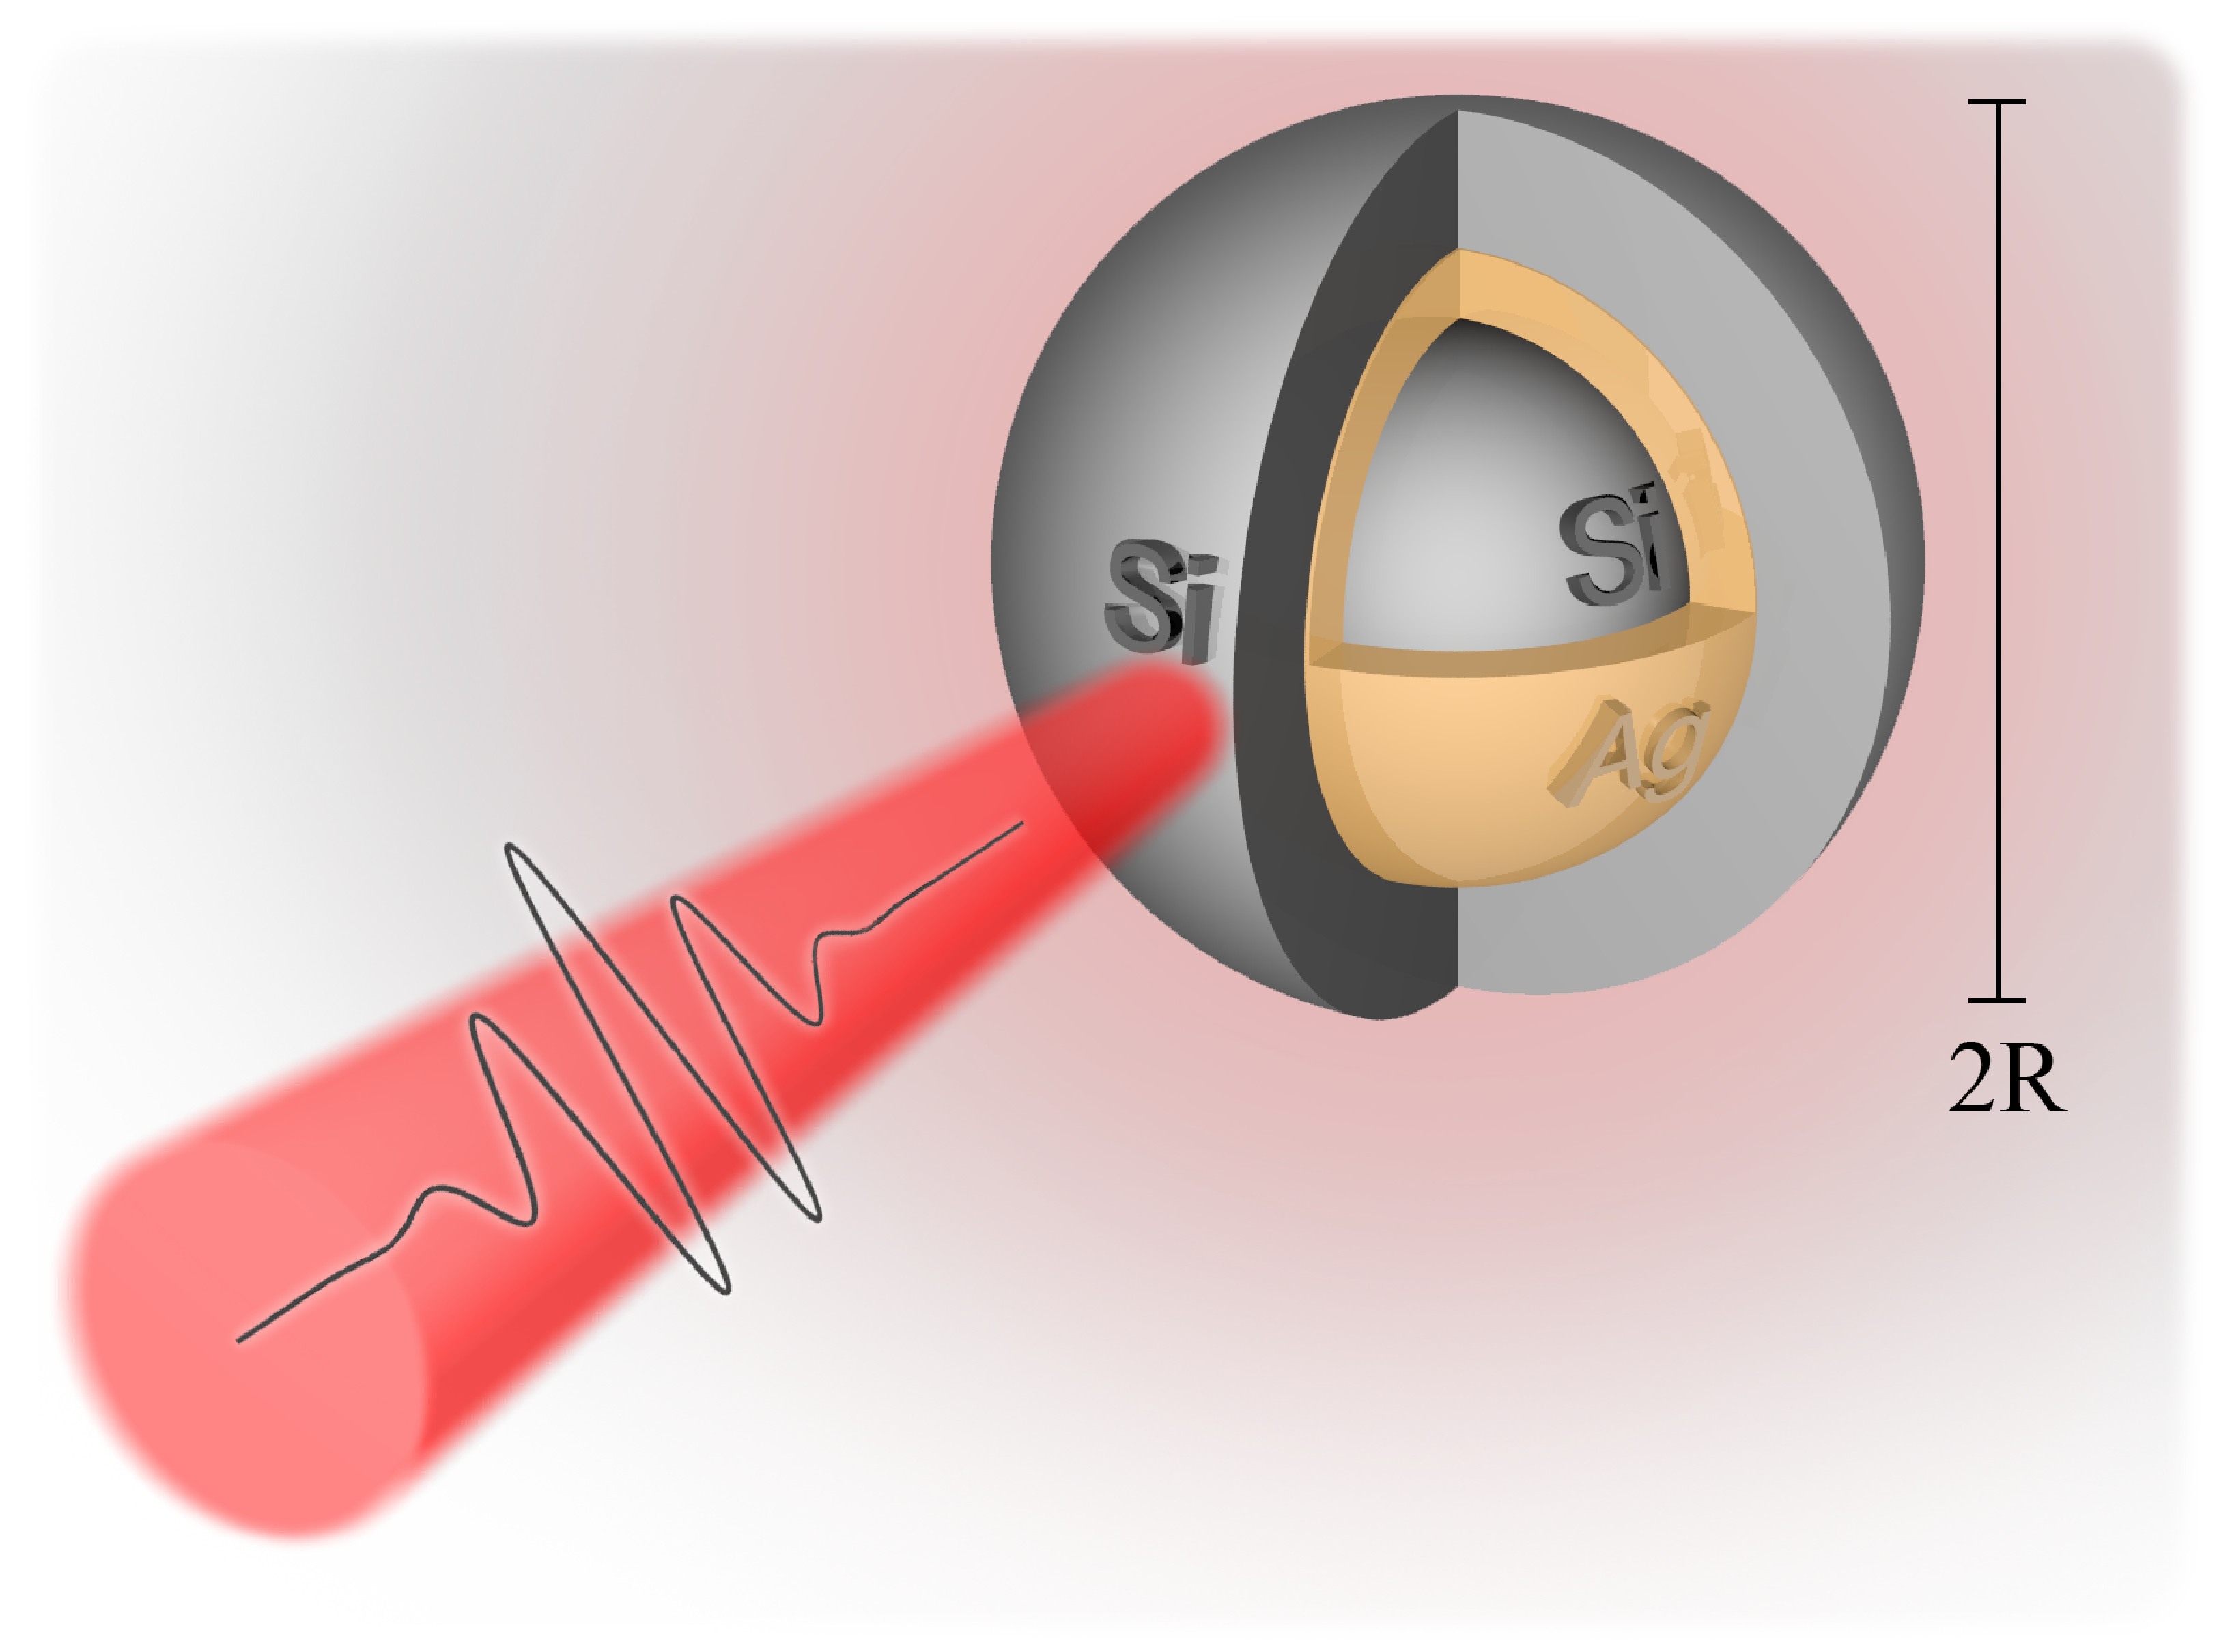
\includegraphics[width=0.4\textwidth]{Fig1}%
    \caption{Shematic view of the simulated $Si/Ag/Si$ particle. 
      \label{fig:geom}
    }%
  }
\end{figure}

The proposed approach can be applied to arbitrary combination of
materials, but to be more specific in what follows we consider
dielectric-metal-dielectric triple-layer $Si/Ag/Si$ spherical particle
illuminated by a plane wave schematically shown in
Fig.~\ref{fig:geom}. In what follows we describe the materials using
experimentally measured parameters from Ref.,\cite{palik-1997}
e.g. at $\lambda = 500$ nm $\epsilon_{Si} = 18.5 + i0.63$ and
$\epsilon_{Ag} = -8.5 + i0.76$.  To optimize the thickness of each
layer we implemented\cite{JADE-web} an adaptive differential
evolution algorithm,\cite{Storn-DE-first-1997} which is called
JADE.\cite{Jingqiao-JADE-2009}  The technical details of the
optimization algorithm were published previously in
Ref.\cite{Ladutenko-2014} We perform Mie calculations using the
Scattnlay software,\cite{Pena-scattnlay-2009,Scattnlay-web} whose
results are verified by a number of other implementations of the Mie
solutions and by commercially available software including CST
Microwave studio\cite{CST-web} and Comsol
Multiphysics.\cite{Comsol-web}

It is a common understanding that, in general, a larger particle has a
larger absorption cross-section, so sphere with the diameter of 1 cm
absorbs more light than any nanoscale sphere. Therefore, it is
practical to employ {\em the absorption efficiency} $Q_{\rm
  abs}=C_{\rm abs}/\pi R^2$, where $R$ is the outer radius of the
particle and $C_{\rm abs}$ is the absorption cross-section.

\begin{figure}[h]
  \center{
    % Use pdfcrop to remove white margins
    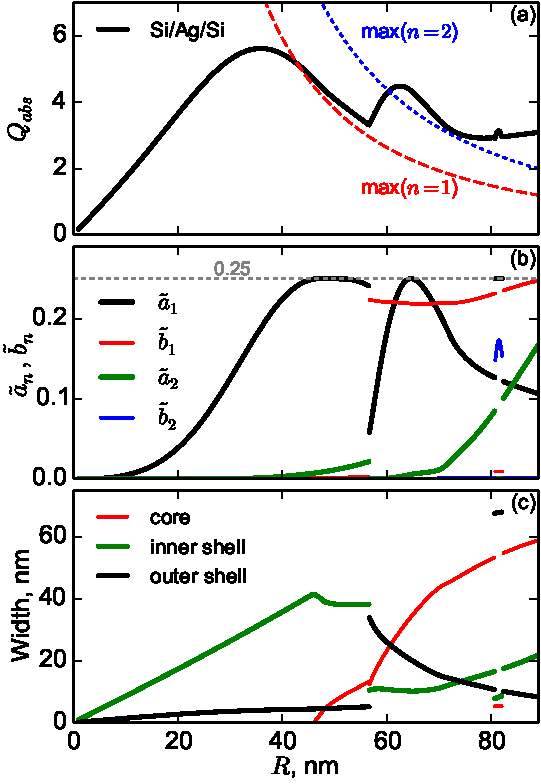
\includegraphics[width=0.45\textwidth]{2015-04-01-Qabs-SiAgSi-overview}%
    \caption{Results of optimization of the absorption efficiency
      for the fixed wavelength of 500~nm. (a) Absorption efficiency
      with the best value achieved for the particle of the
      double-layer Ag/Si design of the radius of 36~nm. Dashed lines
      show theoretical limits for the first channel and second channel
      absorption. The second and third peaks in the absorption
      efficiency curve exceed the theoretical limit for the second
      mode absorption at $R=63$~nm and $R=81$~nm. Local maxima of
      absorption efficiency are additionally marked with arrows. (b)
      Mie absorption coefficients for individual excited modes of the
      optimized structures. (c) Optimized layer thicknesses. For the
      total particle radius below 46~nm the optimizer converges to a
      bi-layer structure, when core size vanishes, and the optimum
      design is a $Ag/Si$ particle. 
      \label{fig:overview}
    }%
  }
\end{figure}
%
In order to study the dependence of the absorption efficiency on the
outer particle size, we run optimization algorithm for different
(fixed) particle outer size, and our optimization parameters are the
radii of internal cores, whereas the target function is the absorption
efficiency. We maximize absorption efficiency at a fixed wavelength of
the incident light (we have chosen $\lambda=500$~nm). We show the
results of our stochastic optimization algorithm in
Fig.~\ref{fig:overview}~(a).  Dashed lines show theoretical absorption
limit of a dipole ($n=1$) and a quadrupole ($n=2$)
resonances,\cite{Tribelsky-2011} which are given as \[Q^{(n)}_{\rm
  abs\ max}=\frac{2n+1}{2q^2},\] where the size parameter $q=2\pi
R/\lambda$, and $n$ is the angular momentum of the mode. Following
Ref.\cite{Fan-2011}, where the authors introduce superscattering for
spherical particles, here we introduce superabsorption regime, when
{\em the ACS is larger than the theoretical limit for absorption by
  strongly excited mode with the highest angular momentum $n$}. In our
parameter space we have modes up to the quadrupole excited ($n=2$),
and in order to get superabsorption our efficiency should be higher
than that of a quadrupole. We clearly see this superabsorption regime
at $R>60$~nm, in Fig.~\ref{fig:overview}~(a).

In Fig.~\ref{fig:overview}~(b) we present the values of Mie absorption
coefficients for individual excited modes in the structure, while
horizontal dashed line shows the theoretical limit (1/4) for each of
them. $\tilde{a}_{1,2}$ are electric dipole and electric quadrupole,
while $\tilde{b}_{1,2}$ are magnetic dipole and magnetic
quadrupole. For small particles, as expected, absorption is dominated
by electric dipole $\tilde{a}_1$.  At $R > 56.6$~nm the optimization
procedure finds that the designs with both electric and magnetic
dipoles have larger ACS than the structure with only the electric
dipole excited. This is why the curves in
Figs.~\ref{fig:overview}~(b,c) experience the discontinuity. Quite
remarkably, in this regime, {\em the combined absorption of the
  electric and magnetic dipoles exceeds the theoretical limit for the
  higher order (quadrupole) mode.}  We also note that there is a very
narrow range of particle sizes, between 80.7~nm and 82.1~nm, where our
analysis finds that the design supporting electric dipole
$\tilde{a}_1$ and magnetic quadrupole $\tilde{b}_2$ has larger ACS,
and this explains two more discontinuities of the curves at the
respective size values.

Fig.~\ref{fig:overview}~(c) shows optimized sizes of layers inside a
multilayer structure. It reveals quite a curious result, that the
dipole branch (i.e. for particle radii below 56.6~nm) has two
parts. For $R<46$~nm the best absorber has just two layers, as the
radius of the core of a triple-layer structure vanishes, and the
particle reduces to $Ag/Si$ core-shell structure.  At $R=46$~nm dipole
channel reaches its theoretical limit (it becomes
$\tilde{a}_1>0.249$).  It appears that the optimizer introduced the
inner $Si$ layer in order to keep $\tilde{a}_1$ near the theoretical
limit as the $R$ increases.  As a side effect, the quadrupole
contribution $\tilde{a}_2$ appears; however, it does not help to reach
superabsorption limit for $n=2$.

Remarkably, the absolute maximum {\em absorption efficiency} is not
reached within the superabsorption regime. Figure~\ref{fig:overview}
shows that the maximum efficiency is achieved for small particle size,
and the ACS is still well below the single channel limit. It appears
that the $Ag/Si$ core-shell nanoparticle with the total radii of
approximately 36~nm is the most efficient absorber among the
considered structures, whose ACS reaches values {\em over 5 times the
  physical cross-section area of the particle}.  From a practical
point of view, it is quite important that the maximum can be reached
in a bi-layer structure, instead of a triple-layer, since it should be
easier and cheaper to fabricate.  At the same time the best absorption
efficiency for larger particles (with $R>60$~nm for provided
materials) can be achieved in superabsorption regime. This may be
important when fabrication of smaller multi-layer particles is not
available.

\begin{figure}[h]
  \center{
    % Use pdfcrop to remove white margins
    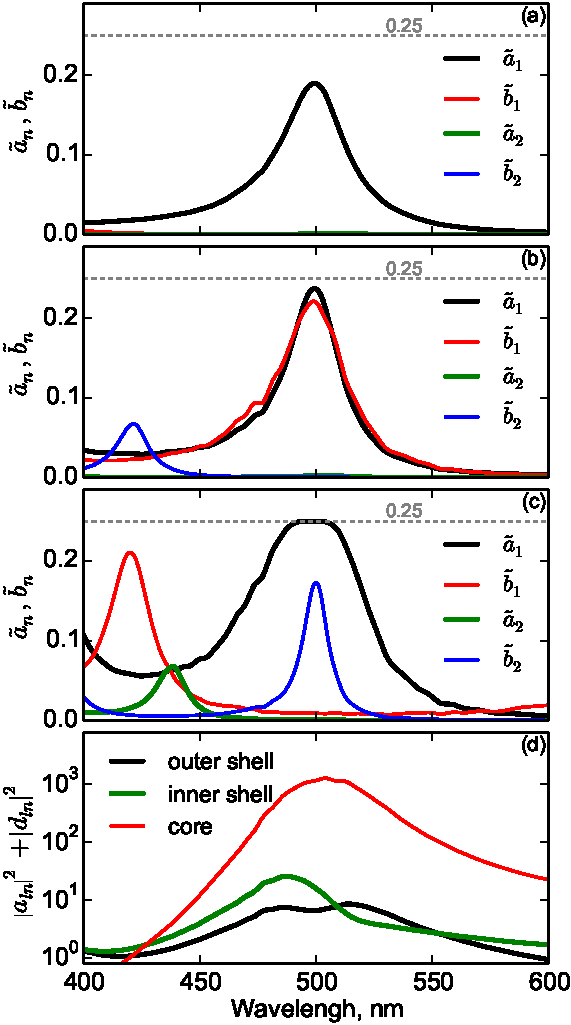
\includegraphics[width=0.45\textwidth]{2015-04-01-SiAgSi-ab-spectra4}%
    \caption{Spectra of Mie absorption coefficients of (a)~efficient
      and (b-c)~superabsorption design. Panel~(d) shows the
      superposition of the squared absolute values of the Mie
      coefficients for electric dipole contribution inside each layer
      of design from panel~(c), which is needed to explain an almost
      flat top of the electric dipole resonance.
      \label{fig:spectra}
    }%
  }
\end{figure}
To study spectral properties of structures with large ACS which we
obtained by the optimization, in Fig.~\ref{fig:spectra} we plot three
different cases for designs that correspond to local maxima of $Q_{\rm
  abs}$ shown in Fig.~\ref{fig:overview}~(a).  As expected, the design
corresponding to the maximum absorption efficiency at $R=36$~nm has a
single electric dipole resonance centered at the target wavelength
$\lambda=500$~nm. Spectra of designs with maxima at $R=63$~nm and
$R=81$~nm have a signature of the superabsorption, i.e. there is an
overlap of several resonances.  We note that these structures have
additional absorption resonances, but they are located far from the
wavelength of interest.  A noticeable feature of
Fig.~\ref{fig:spectra}~(c) is an almost flat top of the electric
dipole resonance. More detailed analysis shows that we have {\em
  excited several electric dipole resonances} with close resonance
frequencies within our multilayer structure. Indeed, if we plot a
superposition of the squares of the absolute values of the Mie
coefficients, which characterize electric energy density stored in
each layer, we find that we excite resonances in all three layers, and
they are slightly offset as shown in
Fig.~\ref{fig:spectra}~(d). Combined effect of these resonances
produces the flat and relatively broadband electric resonance response
shown in Fig.~\ref{fig:spectra}~(c).

\begin{figure}[h]
  \center{
    % Use pdfcrop to remove white margins
    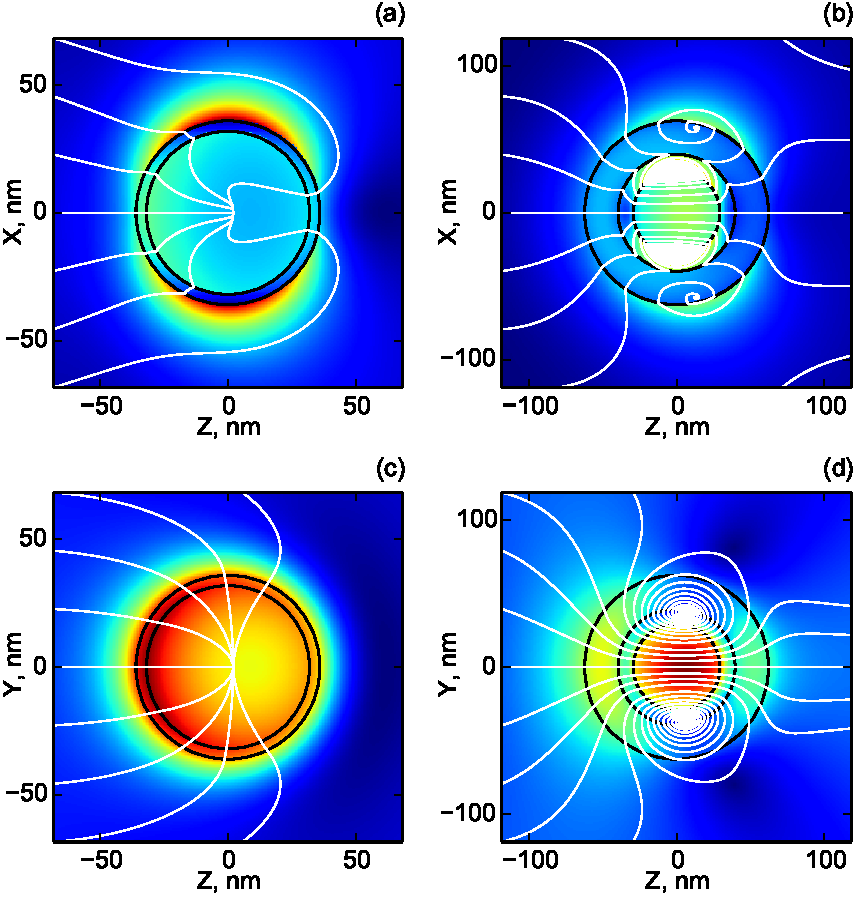
\includegraphics[width=0.47\textwidth]{SiAgSi-flow-R62-YZ-Eabs}%
    \caption{Amplitude of electric field for $R=36$~nm (a,c) and
      superabsorbing designs (b,d) in E-k  (a-b) and H-k (c-d)
      planes normalized to incident wave.  White curves show the
      energy flow streamlines, plane wave comes from the left.
      \label{fig:field}
    }%
  }
\end{figure}
Finally, we present distribution of the amplitude of the electric
field in Fig.~\ref{fig:field} for two designs: with the best
efficiency at $R=36$~nm and in a superabsorbing design with $R=63$~nm.
Using semi-transparent white curves we also plot streamlines of the
Poynting vector which characterize energy flow.  For the effective
design of the absorber, the power from a large cross-sectional area
flows into the particle.  In case of superabsorption regime, we
observe the formation of vortices in the power flow, which make
absorption more efficient as the electromagnetic energy propagates
several times through the absorbing materials.  The reason for the
smaller overall absorption efficiency of a superabsorbing design is
obvious: spatial distribution of the electric field is not uniform
inside the particle and the share of the volume with high absorption
rate in the vortices does not compensate low absorption efficiency in
the regions with small electric field (absorbed power is expressed as
$P_{\rm abs}=\frac{1}{2}\int\sigma \left|E\right|^2dx\,dy\,dz$)

The stochastic algorithm utilized in our approach is very generic and
the optimization can be repeated for any desired wavelength or
wavelength range.  As a result, one can design absorbers with broad
spectra or spectrally-selective absorbers with almost arbitrary
prescribed properties.  One can also achieve broadband performance by
mixing particles whose absorption is optimized for different
wavelengths. We have verified that due to strong localization of
electric dipole field it is possible to design dimers whose absorbing
properties are dominated by the properties of individual particles,
and not by their mutual interaction. As a result, by appropriately
spacing the resonances of individual particles, their mixture will
exhibit a combined broadband response. Providing such an additional
control, this approach complements the case of self-organized
particles of various size and shape, which was experimentally proved
to have a wide absorption band~[ACS-AMI-Liu-2015]. % Reference to the
% paper mentioned with the reviewer in his second comment.
Further control of the absorption spectrum can be achieved by
arranging our spherical structures in a periodic and non-periodic
arrays.

We note, that using this algorithm, one can optimize not
only absorbtion efficiency, but also other parameters that may be
desired for some applications. As an example we reproduce some of the
results from the work of Estakhri and Al\`u,\cite{Alu-2014} where
authors aim to design absorbers with small scattering cross-section,
and we provide a number of new optimized designs. The efficiency in
the Ref.\cite{Alu-2014} is defined as the ACS normalized to
scattering cross-section. Initially, we set the total value of the
absorbed power with cross-section of $\alpha_{\rm
  abs}=\frac{3\lambda^2}{8\pi}$ and keep the outer radius of the
particle fixed. In this case the optimization gives a result similar
to the structure with contributing harmonics TM${_1}$ and TE$_1$ from
Ref.\cite{Alu-2014}  For $\epsilon_1 = 1.29+i0.01$, $\epsilon_2 =
-10.37+ i0.35$, and $\epsilon_3=8.4+i2.33$ as material parameters we
obtained radii $\{a_{c1},a_{c2},a_3\}=\{0.142,0.166,0.194\}\lambda$
and scattering-normalized absorption efficiency $\eta_{\rm
  abs}^{(\alpha)} =7.65$ which corresponds to $\eta_{\rm
  abs}^{(\alpha)} =7.1$ from the original work.\cite{Alu-2014}
However, if we set the optimizer to keep high level of absoption
efficiency $Q_{\rm abs} \approx 5$ the particle becomes much smaller
and the size of the outer layer vanishes
$\{a_{c1},a_{c2}\}=\{0.00635,0.00747\}\lambda$ resulting in $\eta_{\rm
  abs}^{(Q)} =544$.  It means that this small particle still absorbs
five times its phisical size with a very large scattering-normalized
absorption efficiency.

% Moreover, it is easy to set the optimizer to keep $\eta_{\rm abs}
% \approx 100$ or $\eta_{\rm abs} \approx 1000$, resulting
% $\{a_{c1},a_{c2}\}=\{0.0112,0.0131\}\lambda$, $Q_{\rm abs} = 8.65$
% or $\{a_{c1},a_{c2}\}=\{0.0052,0.0061\}\lambda$, $Q_{\rm abs} =
% 3.26$ respectively.


In conclusion, we introduce and study the effect of superabsorption,
when the absorption cross-section of the nanoparticle can reach the
theoretical limit for several modes at the same frequency. This
becomes possible when several resonant modes of the structure overlap
at the same frequency, and this regime can be achieved in multilayer
nanoparticles. Moreover, quite unexpectedly we find that the most
efficient absorbers, which are characterized by enhanced absorption
efficiencies, are smaller nanoparticles working in a single mode
regime. We present their spectral characteristics and field structure.
It is interesting to note that a similar conclusion was made by Miller
et al.\cite{Miller-2014} for extinction of arbitrary particles: small
size with only dipole response is preferable for geometric volume
normalized efficiency.


  Thanks to David A. Powell for his contribution to the analysis of
  the spectrum feature.  AEM and IVS acknowledge the support from the
  Australian Research Council through Future Fellow and Discovery
  project schemes. OPR is grateful to Consejo Nacional de Ciencia y
  Tecnolog\'{i}a (Mexico) for financing a short stay at Universidad
  Autónoma de Puebla, Mexico.  KSL and PAB thank the Ministry of
  Education and Science of the Russian Federation and Government of
  the Russian Federation (Grant 074-U01) for the financial support.




% \begin{figure}[h]
% \centering
%   \includegraphics[height=3cm]{example}
%   \caption{An example figure caption}
%   \label{fgr:example}
% \end{figure}

% \begin{figure*}
%  \centering
%  \includegraphics[height=3cm]{example2}
%  \caption{An image from the \textit{Physical Chemistry Chemical Physics} cover gallery, set as a double-column figure.}
%  \label{fgr:example2col}
% \end{figure*}





%The \balance command can be used to balance the columns on the final page if desired. It should be placed anywhere within the first column of the last page.

\balance

%If notes are included in your references you can change the title from 'References' to 'Notes and references' using the following command:
%\renewcommand\refname{Notes and references}

%%%REFERENCES%%%
\scriptsize{
%\bibliography{rsc} %You need to replace "rsc" on this line with the name of your .bib file
\bibliography{2015-Ladutenko-Qabs}
\bibliographystyle{rsc} } %the RSC's .bst file

\end{document}
